%%% Greedy 97, 125_plot.dat, profit only
%%% E.g. order 14. altough it has a profit of 10 which is above average, it takes 114 timelots and occupies 3 slots for the basically the whole schedule. Altough they have a bit less profit, there are many orders which only take 3 surface and are way shorter to process 
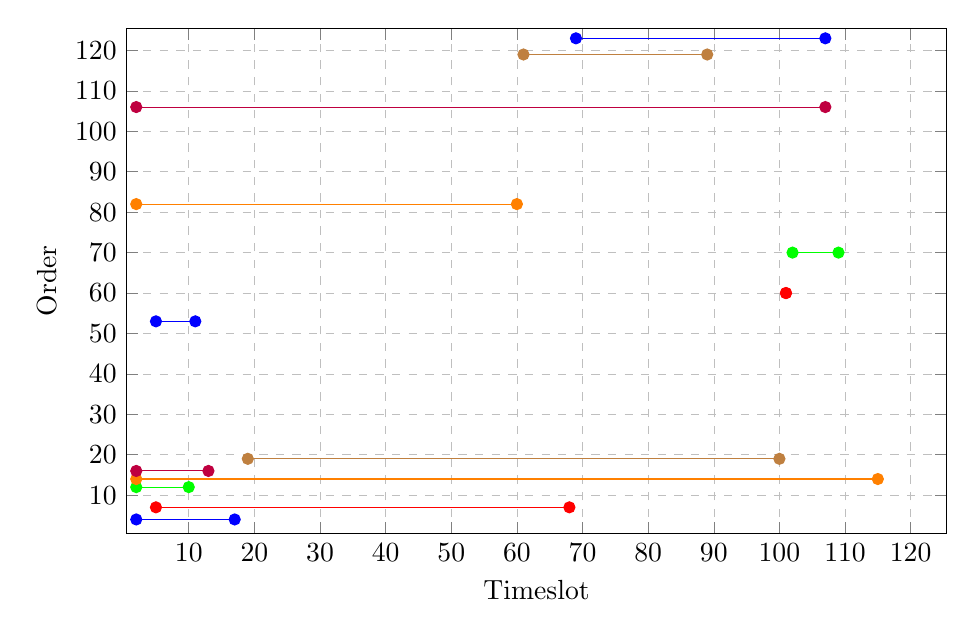
\begin{tikzpicture}
\begin{axis}[
    xlabel={Timeslot},
    ylabel={Order},
    xmin=0.5, xmax=125.5, 
    ymin=0.5, ymax=125.5, 
    xtick={10,20,30,40,50,60,70,80,90,100, 110, 120},
    ytick={10,20,30,40,50,60,70,80,90,100, 110, 120},
    grid=both,
    grid style={line width=.1pt, draw=gray!10},
    major grid style={line width=.2pt, draw=gray!50},
    legend pos=north east,
    ymajorgrids=true,
    xmajorgrids=true,
    grid style=dashed,
     width=12cm,
     height=8cm,
]
\addplot[color=blue, mark=*] coordinates {(2, 4) (17, 4)};
\addplot[color=red, mark=*] coordinates {(5, 7) (68, 7)};
\addplot[color=green, mark=*] coordinates {(2, 12) (10, 12)};
\addplot[color=orange, mark=*] coordinates {(2, 14) (115, 14)};
\addplot[color=purple, mark=*] coordinates {(2, 16) (13, 16)};
\addplot[color=brown, mark=*] coordinates {(19, 19) (100, 19)};
\addplot[color=blue, mark=*] coordinates {(5, 53) (11, 53)};
\addplot[color=red, mark=*] coordinates {(101, 60) (101, 60)};
\addplot[color=green, mark=*] coordinates {(102, 70) (109, 70)};
\addplot[color=orange, mark=*] coordinates {(2, 82) (60, 82)};
\addplot[color=purple, mark=*] coordinates {(2, 106) (107, 106)};
\addplot[color=brown, mark=*] coordinates {(61, 119) (89, 119)};
\addplot[color=blue, mark=*] coordinates {(69, 123) (107, 123)};
\end{axis}
\end{tikzpicture}